% Template for Cogsci submission with R Markdown

% Stuff changed from original Markdown PLOS Template
\documentclass[10pt, letterpaper]{article}

\usepackage{cogsci}
\usepackage{pslatex}
\usepackage{float}
\usepackage{caption}

% amsmath package, useful for mathematical formulas
\usepackage{amsmath}

% amssymb package, useful for mathematical symbols
\usepackage{amssymb}

% hyperref package, useful for hyperlinks
\usepackage{hyperref}

% graphicx package, useful for including eps and pdf graphics
% include graphics with the command \includegraphics
\usepackage{graphicx}

% Sweave(-like)
\usepackage{fancyvrb}
\DefineVerbatimEnvironment{Sinput}{Verbatim}{fontshape=sl}
\DefineVerbatimEnvironment{Soutput}{Verbatim}{}
\DefineVerbatimEnvironment{Scode}{Verbatim}{fontshape=sl}
\newenvironment{Schunk}{}{}
\DefineVerbatimEnvironment{Code}{Verbatim}{}
\DefineVerbatimEnvironment{CodeInput}{Verbatim}{fontshape=sl}
\DefineVerbatimEnvironment{CodeOutput}{Verbatim}{}
\newenvironment{CodeChunk}{}{}

% cite package, to clean up citations in the main text. Do not remove.
\usepackage{cite}

\usepackage{color}

% Use doublespacing - comment out for single spacing
%\usepackage{setspace}
%\doublespacing


% % Text layout
% \topmargin 0.0cm
% \oddsidemargin 0.5cm
% \evensidemargin 0.5cm
% \textwidth 16cm
% \textheight 21cm

\title{Children's social referencing reflects sensitivity to graded uncertainty}


\author{{\large \bf Emily  Hembacher} \\ \texttt{ehembach@stanford.edu} \\ Department of Psychology \\ Stanford University \And {\large \bf Benjamin deMayo} \\ \texttt{bedemayo@stanford.edu} \\ Department of Psychology \\ Stanford University \And {\large \bf Michael C. Frank} \\ \texttt{mcfrank@stanford.edu} \\ Department of Psychology \\ Stanford University}

\begin{document}

\maketitle

\begin{abstract}
The ability to monitor epistemic uncertainty is critical for active
learning. However, we still know little about young children's ability
to monitor epistemic uncertainty and coordinate information-gathering
behaviors on its basis. Here we examined a spontaneous behavioral
reaction to uncertainty, social referencing, during a word learning task
among preschoolers. Children ages 2-5 were asked to place a target
object in a bucket after hearing the experimenter produce a label for
the target. We manipulated referential ambiguity through the number of
objects present and their familiarity: in Experiment 1, when there were
two unfamiliar objects and an unfamiliar label, the referent was
unclear; when there were two familiar objects, or only one novel or
familiar object, the referent was known or could be inferred. In
Experiment 2, there were either two novel objects, two familiar objects,
or one familiar and one novel object, in which case the referent could
be inferred using the mutual exclusivity principle. Across Experiments 1
and 2, children looked up to the experimenter more often while executing
a decision about which object to place in the bucket when there were two
novel objects and thus uncertainty about the object-label mapping, and
they did so while planning their decision as well in Experiment 1. In
Experiment 2, children also referenced the experimenter more on mutual
exclusivity trials, but only when the experimenter did not gaze at the
object as she labeled it, suggesting that children's social referencing
is sensitive to graded evidence.

\textbf{Keywords:}
social referencing; help seeking; word learning; uncertainty.
\end{abstract}

Human learning can be characterized as a problem of detecting and
reducing epistemic uncertainty. Being able to detect uncertainty in our
own knowledge allows us to reduce that uncertainty by seeking
disambiguating information or communicating uncertainty to social
partners. Uncertainty monitoring may be particularly critical early in
life, when children are tasked with learning their native language, the
social and cultural structure of their world, and the causal properties
of their environment. However, there has been mixed evidence about the
extent to which young children are conscious of their own knowledge and
mental states, and their ability to act on this meta-awareness
(Schneider, 2008; Sodian, Thoermer, Kristen, \& Perst, 2012). This
raises questions about how active young children's learning is; do
preschool-aged children monitor uncertainty and guide their learning
behaviors on the basis of this monitoring, or is early learning better
characterized as a process of integrating information that is largely
generated externally, for example, by social partners who act as
teachers (Csibra \& Gergely, 2006)?

Research on children's uncertainty monitoring within a metacognitive
framework has shown that children fail at reporting on their ongoing
thoughts (J. H. Flavell, Green, Flavell, Harris, \& Astington, 1995) and
are inconsistently able to report explicitly on their confidence in
their knowledge (Hembacher \& Ghetti, 2014; Lyons \& Ghetti, 2013;
Paulus, Proust, \& Sodian, 2013). For example, 3-year-olds report being
equally sure about correct and incorrect responses in a memory task
(Hembacher \& Ghetti, 2014). There is also protracted development
throughout childhood of other metacognitive abilities, such as
estimating future performance (Destan, Hembacher, Ghetti, \& Roebers,
2014; Lipowski, Merriman, \& Dunlosky, 2013) and selectively allocating
learning time to difficult or less-well-learned materials (Metcalfe \&
Finn, 2013). However, most of these studies have relied upon explicit
reports of uncertainty or learning progress. It is possible that
children are able to act upon their environment and their own knowledge
on the basis of uncertainty monitoring prior to their ability to bring
it fully into consciousness or organize an explicit response about it.

In support of this possibility, several studies have shown that infants
and toddlers engage in spontaneous information-seeking behaviors
selectively in response to epistemic uncertainty. For example, Call and
Carpenter (2001) had 2-year-olds choose between several tubes to find a
hidden sticker. They found that the toddlers were more likely to peek
inside a tube before choosing when they had not seen the baiting of the
tubes compared to when they had, suggesting they were aware of their
ignorance and managed to delay their response until they had a good
answer. In another study, Goupil, Romand-Monnier, \& Kouider (2016)
found that 20-month-olds were more likely to seek help by looking at
their parents when they were unable to respond accurately in a memory
task. These implicit measures may better capture uncertainty signals by
bypassing the need to orchestrate an explicit response, even a
non-verbal one. Thus, examining spontaneous information-gathering
behaviors may resolve remaining questions about young children's ability
to monitor uncertainty, including uncertainty generated by graded
evidence in different learning scenarios.

Here, we focus on the role of uncertainty in guiding social referencing
--- one form of information gathering --- during word learning. One of
the cues children have available to them when learning object-label
mappings is the direction of a speaker's gaze, as people tend to look at
objects they are referring to. By the second year of life infants follow
a speaker's gaze and map labels to objects on the basis of gaze
direction (Brooks \& Meltzoff, 2002). There is also evidence that
infant's propensity for gaze-following predicts later language
development (Brooks \& Meltzoff, 2008), highlighting the importance of
this behavior for learning.

Although gaze-following is clearly critical for word-object mapping, at
any given moment, there are many stimuli in the visual field that
compete for attention. In some cases, a listener may be required to
disengage from a salient or informative stimulus in order to reference a
speaker's gaze direction to resolve referential ambiguity. Thus, it may
be optimal to follow a speaker's gaze only when disambiguating
information is needed, which would require the listener to monitor her
own uncertainty. Investigating the selectivity of gaze-following and
social referencing in general may be a particularly useful case study of
uncertainty monitoring processes for several reasons. First of all,
social referencing is a ubiquitous spontaneous behavior across the
lifespan, and thus does not have to be prompted and is ecologically
valid. Second of all, looking is a continuous measure, allowing us to
determine whether it, and therefore the monitoring system, is sensitive
to graded uncertainty.

Do infants and children follow a speaker's gaze regardless of the need
for disambiguation, or do they selectively follow gaze when the referent
of a word is unknown? Vaish, Demir and Baldwin (2011) investigated this
question with 13- and 18-month-olds infants. Infants sat across from an
experimenter who produced a label (e.g., ``a modi!) in the presence of
one or two objects. They found that infants looked up to the
experimenter more often when there were two objects present, and the
referent was thus ambiguous. They interpret this to mean that infants
recognize when they need disambiguating information and reference gaze
accordingly. In addition, when only one object was present, infants
successfully mapped the new label to the object, as confirmed in a
comprehension test in which children had to place a named object in a
bucket. In sum, infants appear to selectively reference a speaker when
uncertainty about the referent of a label is high.

The present research adapts Vaish et al. to examine whether
preschool-aged children's social referencing is sensitive to uncertainty
based on referential ambiguity, and whether it reflects graded
uncertainty about a word-object mapping. In addition to measuring
children's looking during the labeling event itself, we measured looking
across an event in which children heard a label and then were asked to
select the corresponding object and put it in a bucket. We predicted
that children might selectively reference their interlocutor on the
basis of uncertainty while planning and executing their decision in
addition to during the labeling itself, as social information might be
expected to be available throughout the mapping and decision processes.

\begin{CodeChunk}
\captionsetup{width=0.8\columnwidth}\begin{figure}[h]

{\centering 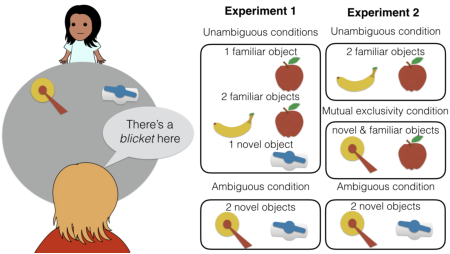
\includegraphics{figs/image_design-1} 

}

\caption[Study design for Experiments 1 and 2]{Study design for Experiments 1 and 2.}\label{fig:image_design}
\end{figure}
\end{CodeChunk}

\section{Experiment 1}\label{experiment-1}

In Experiment 1, we examined whether children would reference a speaker
more often when there was referential ambiguity associated with a label
she produced. We were interested not only in children's referencing of
gaze direction during the labeling itself, but referencing of the
speaker after the labeling event while children made a decision about
which object was the intended referent. We predicted that children would
seek confirmation of the accuracy of their choice from the speaker when
they were uncertain, perhaps expecting an emotional reaction or explicit
approval, in addition to seeking gaze direction information during
labeling. We will refer to looks during and after labeling as social
referencing, as the looks could reflect different types of information
gathering.

We had children sit across from an experimenter who labeled an object on
the table between them (Figure \ref{fig:design}). Across trials, there
were either one or two objects, which were either familiar or unfamiliar
to the child. We expected children to be uncertain about the label's
referent only on trials with two unfamiliar objects. After labeling an
object, the experimenter asked the child to place the named object in a
bucket. We measured the number of times the child looked up to the
experimenter's face during four discreet phases of the trial: the
labeling event (\emph{label} phase), the sliding of the object(s) into
the child's reach (\emph{slide} phase), the time before the child
touched an object once they were within reach (\emph{planning} phase),
and the time between touching an object and dropping it in the bucket
(\emph{response} phase).

We predicted that children would look to the experimenter more often on
two-object novel trials compared to the other three trial types during
the labeling, planning, and response phases, which would indicate that
they recognized the need for disambiguating information. We did not
predict that children would look more for these trial types during the
slide phase, when they would likely be looking at the objects
themselves.

\subsection{Methods}\label{methods}

\subsubsection{Participants}\label{participants}

We recruited a planned sample of 80 children ages 2-5 years from the
Children's Discovery Museum in San Jose,
California\footnote{Planned sample size, exclusion criteria, and analysis plan preregistered at https://osf.io/y7mvt/}.
The sample included 20 2-year-olds (mean age 31.71 months), 20
3-year-olds (mean age 42.65 months), 20 4-year-olds (mean age 55.85
months), and 20 5-year-olds (mean age 65.11 months). An additional 20
children participated but were removed from analyses because they heard
English less than 75\% of the time at home (\emph{n} = 10), because they
were unable to complete at least half of the trials in the task
(\emph{n} = 4), because of parental interference (\emph{n} = 1), or due
to experimenter or technical errors (\emph{n} = 5).

\subsubsection{Stimuli and Design}\label{stimuli-and-design}

In this task, children were presented with one or two objects, heard a
label, and were asked to put the labeled object in a bucket. Half of the
objects were selected to be familiar to children (e.g., a cow) and half
were selected to be novel (e.g., a nozzle). There were four trial types:
one-familiar, one-novel, two-familiar, and two-novel. There were three
trials of each type, for a total of twelve trials, and trial types were
presented sequentially in an order that was counterbalanced across
participants. The assignment of individual objects to trial types was
counterbalanced. On familiar trials, the familiar label for the target
object was used (e.g., ``cow''). On novel trials, a novel label was used
(e.g., ``dawnoo'').

The critical manipulation was of referential ambiguity; on one-familiar
and two-familiar trials, there was no referential ambiguity, as children
were expected to be certain about the objects and their labels.
Similarly, on one-novel trials, children were expected to be certain
about the label referent as there was only one option. However, on
two-novel trials, the referent was ambiguous, as the novel label could
apply to either novel object.

\subsubsection{Procedure}\label{procedure}

Throughout the study, the child sat at one end of a large circular
table, and the experimenter stood at the opposite end. Each trial of the
task proceeded as follows: the experimenter placed one or two objects on
the left and/or right sides of the table, out of reach of the child so
that the child could not interact with the toys during the labeling
event. For one-object trials, the location of the object (left or right)
alternated between trials. After placing the objects, the experimenter
said ``Hey look, there's a (target) here.'' The experimenter gazed at
the center of the table rather than the object she was labeling because
we wanted to preserve the referential ambiguity throughout the trial.
The experimenter waited approximately two seconds (based on a visual
metronome placed within view) before saying, ``Can you put the (target)
in the bucket?'' She then pushed the object(s) forward within reach of
the child, and placed a plastic bucket in the center of the table, also
within reach of the child. Prior to the twelve experimental trials,
there were two training trials: a one-familiar trial and a two-familiar
trial, to acquaint the child with the procedure. A camera placed to the
side of the experimenter captured the participant's face, so that
looking behavior could be coded from video.

\subsubsection{Coding procedure}\label{coding-procedure}

Videos were coded using DataVyu software (\url{http://datavyu.org}).
First, each trial was divided into four temporal phases: a \emph{label}
phase, which began at the utterance of the target label and ended when
the experimenter began to slide the objects, a \emph{slide} phase, which
encompassed the sliding of the objects into the child's reach, a
\emph{planning phase}, which began at the end of the slide and ended
when the child touched an object, and a \emph{response} phase, which
began when the child touched an object and ended when the child released
the object into the bucket. After onsets and offsets of these phases had
been coded, the coder recorded the number of looks the child made to the
experimenter's face during each phase. We opted to code the number of
looks rather than the duration of looks because we felt that looks from
the stimuli to the experimenter's face and vice versa might allow
children to integrate social and nonsocial information to solve the
problem of reference. Vaish, Demir and Baldwin found that both the
number of looks and the duration of looks were sensitive to referential
ambiguity among infants. A second coder coded the number of looks for a
quarter of the trials for each participant to establish reliability. For
Experiment 1, \#\#\% of trials were given the same number of looks by
both coders. For Experiment 2, \#\#\% of trials were given the same
number of looks by both coders.

\subsection{Results and Discussion}\label{results-and-discussion}

\begin{CodeChunk}
\begin{figure*}[h]

{\centering 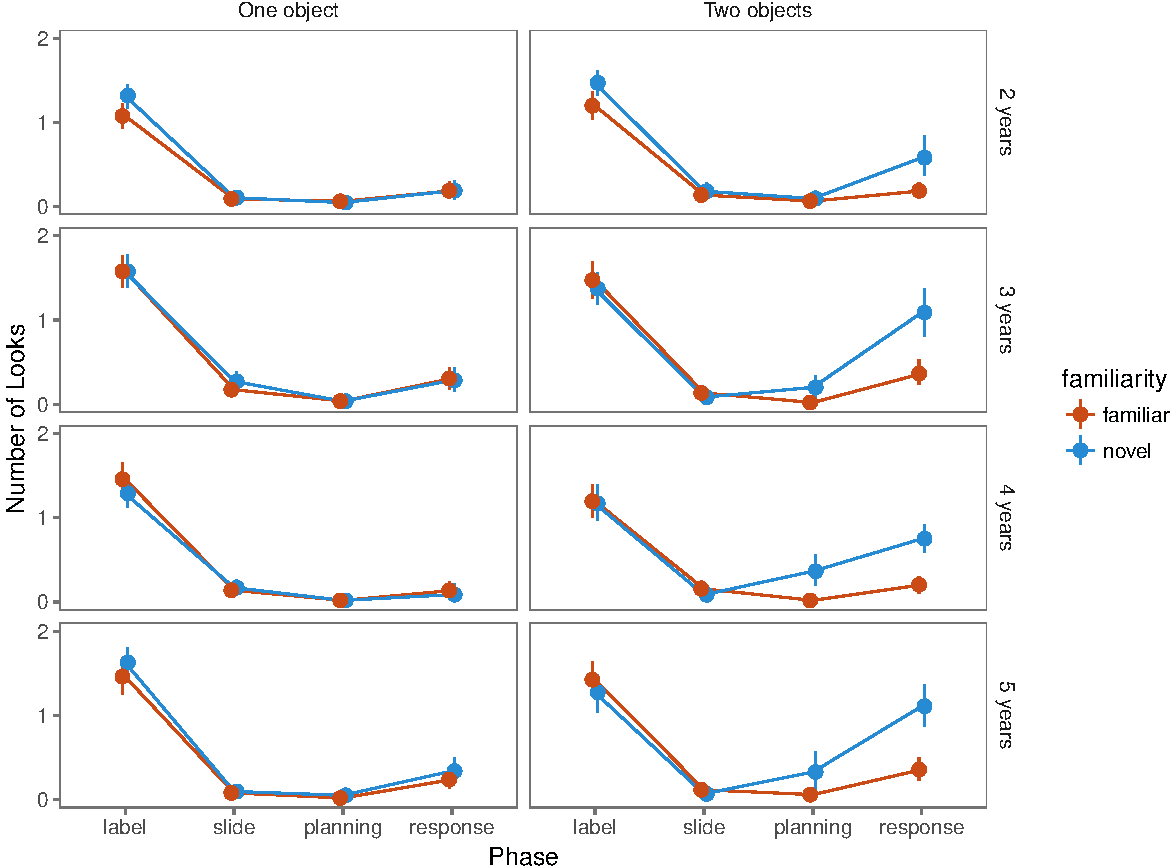
\includegraphics{figs/results_e1-1} 

}

\caption[Results of Experiment 1]{Results of Experiment 1. Number of looks to the experimenter across phases and conditions. Error bars are 95 percent confidence intervals.}\label{fig:results_e1}
\end{figure*}
\end{CodeChunk}

Descriptive results of Experiment 1 are presented in Figure
\ref{fig:results_e1}. To test our prediction that referential ambiguity
(i.e., having two novel objects) would produce more social referencing,
we fit mixed-effects linear regression models separately for each phase
with the following structure:
\texttt{number\ of\ looks\ \textasciitilde{}\ number\ of\ objects\ *\ familiarity\ *\ age\ in\ months\ +\ (number\ of\ objects\ +\ familiarity\ \textbar{}\ SID)}.
A single model with phase as a factor did not converge.

We did not find any main or interactive effects of number of objects,
familiarity, or age on number of looks during the label phase or the
slide phase. However, we found an interactive effect of number of
objects and familiarity during the planning (\(\beta\) = 0.21, \emph{p}
\textless{} .001) and response phases (\(\beta\) = 0.6, \emph{p}
\textless{} .001), such that 2-novel trials were associated with more
looking. There was no interaction with age in either
phase\footnote{Code and data available with full regression model results at https://github.com}.
In summary, children ages 2-5 looked to the experimenter more often when
planning and executing a response under uncertainty. These results
suggest that chidlren were aware that they did not have sufficient
knowledge to answer independently, and they attempted to resolve their
uncertainty using social referencing. We did not find the expected
effect of referential ambiguity in the label phase. There are a number
of reasons we might have observed this null effect. One possibility is
that children failed to predict that they would need more information
until later in the trial, when they were actually faced with planning
and executing a decision. Another possibility is that children's looking
was at ceiling during the labeling phase, perhaps because children look
at someone who is speaking regardless of the need for referential
disambiguation. A third possibility is that this is an artifact of our
design, in which the experimenter gazed at the center of the table
rather than the referent of her label. Children may have realized that
the experimenter's gaze direction during labeling was not a source of
disambiguating information. Experiment 2 tests this possibility and
examines whether children's social referencing is sensitive to graded
uncertainty.

\section{Experiment 2}\label{experiment-2}

Experiment 2 was designed to replicate Experiment 1 and to investigate
whether children's social referencing is sensitive to uncertainty based
on graded evidence in addition to the presence or absence of knowledge.
Since we did not observe any difference between the one-familiar and
one-novel trials, we eliminated single-object trials, leaving the
2-familiar and 2-novel trials. In addition to these trials, we added
1-novel-1-familiar trials to examine social referencing patterns when 2
objects are present and an unfamiliar label is produced, but the label
referent can be deduced through the principle of mutual exclusivity. We
expected that if children are sensitive to graded evidence, mutual
exclusivity trials would generate intermediate levels of uncertainty
compared to novel or familiar trials. On the other hand, if children
merely monitor the presence or absence of relevant information, they
might treat mutual exclusivity trials as familiar trials, given that 3-
to 4-year-olds are generally successful in solving the problem of
reference using mutual exclusivity(Markman, Wasow, \& Hansen, 2003).

In addition, we manipulated between participants whether or not the
experimenter's gaze during labeling was informative (she gazed at either
the referent of her label or the center of the table), allowing us to
determine whether children selectively reference gaze during labeling
when gaze is expected to be informative. The manipulation of
informativity of gaze during labeling also meant that participants in
the referential gaze condition had an additional referential cue, which
might decrease uncertainty in the remainder of the trial.

In Experiment 1, we did not observe an effect of age on looking. Thus,
we restricted the current sample to 3- and 4-year-olds.

\subsection{Methods}\label{methods-1}

\subsubsection{Participants}\label{participants-1}

We recruited a planned sample of 80 children ages 3-4 years from the
Children's Discovery Museum in San Jose,
California\footnote{Planned sample size, exclusion criteria, and analysis plan preregistered at https://osf.io/y7mvt/}.
The sample included 40 3-year-olds (mean age 42.89 months) and 40
4-year-olds (mean age 53.47 months). An additional 20 children
participated but were removed from analyses because they heard English
less than 75\% of the time at home (\emph{n} = 9), because they were
unable to complete at least half of the trials in the task (\emph{n} =
7), or due to experimenter or technical errors (\emph{n} = 4).

\subsubsection{Stimuli and Design}\label{stimuli-and-design-1}

The stimuli and design were similar to Experiment 1, except that we
eliminated 1-object trials. Instead, we included three trial types:
2-familiar (``familiar''), 2-novel (``novel''), and 1-novel-1-familiar
(``mutual exclusivity''). There were four of each trial type, totaling
twelve trials. In addition, we manipulated the experimenter's gaze
behavior between participants. For half of the participants, she looked
at the center of the table on every trial; for the remaining half, she
looked at the object she referred to on every trial.

\subsubsection{Procedure}\label{procedure-1}

The procedure was identical to Experiment 1, except that there were
three practice trials rather than two, so that children could experience
every trial type.

\subsection{Results and Discussion}\label{results-and-discussion-1}

\begin{CodeChunk}
\begin{figure*}[h]

{\centering 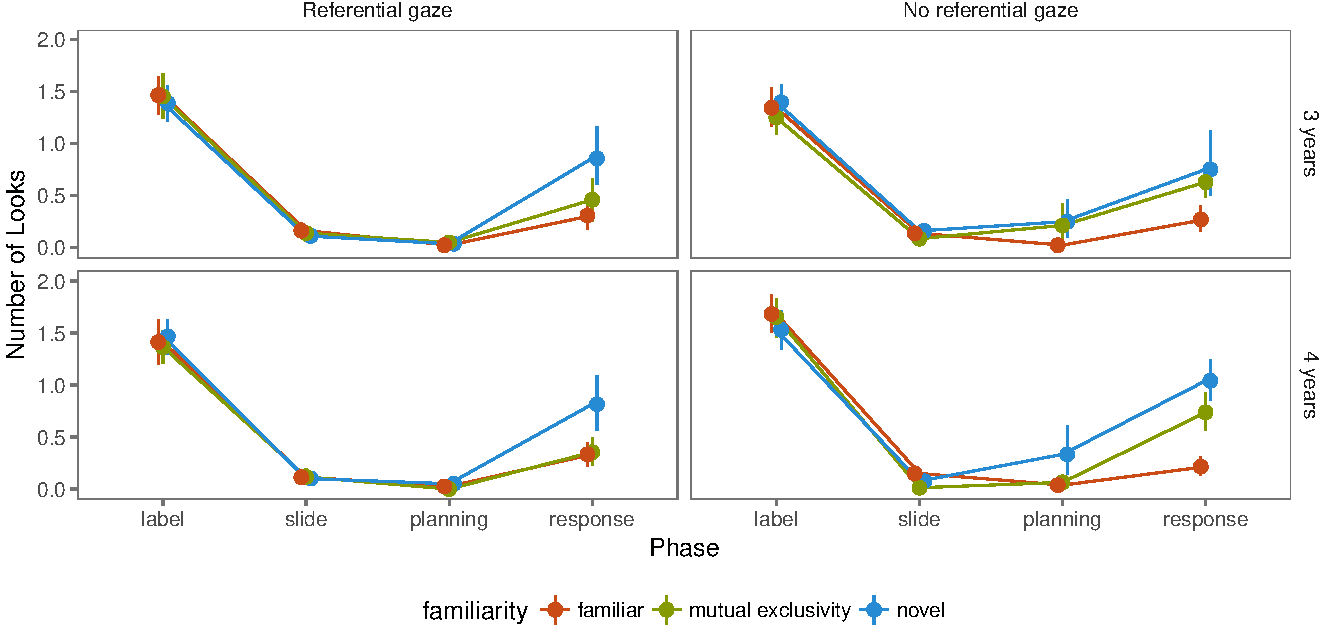
\includegraphics{figs/results_e2-1} 

}

\caption[Results of Experiment 2]{Results of Experiment 2. Number of looks to the experimenter across phases and conditions. Error bars are 95 percent confidence intervals.}\label{fig:results_e2}
\end{figure*}
\end{CodeChunk}

The descriptive results of Experiment 2 are presented in Figure
\ref{fig:results_e2}. To quantify the main and interactive effects of
familiarity, gaze informativity, phase, and age on social referencing,
we fit a mixed-effects linear regression model with the following
structure:
\texttt{number\ of\ looks\ \textasciitilde{}\ familiarity\ *\ age\ in\ months\ *\ gaze\ *\ phase\ +\ (familiarity\ \textbar{}\ SID)}.

We were interested in several questions. First, do children reference a
speaker more often when the objects and label are novel? As in
Experiment 1, there was an interaction of phase with familiarity such
that the response phase of novel trials was associated with
significantly more looks (\(\beta\) = 0.51, \emph{p} \textless{} .001).
However, we did not observe such an interaction for the planning phase.

We were also interested in whether mutual exclusivity trials would
elicit an intermediate amount of social referencing. We observed a
three-way interaction of familiarity, gaze, and phase, such that the
response phase of mutual exclusivity trials in the no-referential-gaze
condition was associated with significantly more looks (\(\beta\) =
0.39, \emph{p} \textless{} .01). In sum, mutual exclusivity trials were
associated with greater looking during the response phase when the
experimenter provided informative gaze compared to when she did not.
This is intriguing given that children should be able to solve mutual
exclusivity trials without gaze information. Instead, it seems that they
remain somewhat uncertain while executing a decision if mutual
exclusivity is their only cue to reference, but this uncertainty is
resolved if the experimenter gazes at the correct object during
labeling. This provides evidence for sensitivity to graded evidence.

Finally, we observed a four-way interaction such that the response phase
of novel trials in the gaze condition was associated with more looking
with increasing age (\(\beta\) = 0.06, \emph{p} \textless{} .01),
suggesting that children may become more selective in their social
referencing as they get older. It may be that children improve in their
ability to monitor the need for disambiguating information, or they may
become more likely to recognize that social information can be a source
of disambiguation. However, the interaction with age should be
interpreted with caution as we did not find an interaction with age in
Experiment 1.

Lastly, we did not find selective social referencing during the label
phase, even when referential gaze was available. This rules out the
possibility that children were less selective during this phase because
they realized that gaze direction was not informative.

\section{General Discussion}\label{general-discussion}

Preschoolers quickly learn new concepts, rules, and language, often with
minimal exposure. They also actively explore and ask questions in ways
that seem targeted to maximize learning (Chouinard, Harris, \& Maratsos,
2007; L. E. Schulz \& Bonawitz, 2007). However, we still have an
incomplete understanding of young children's ability to monitor their
own mental states, in particular, their epistemic uncertainty. Do
children monitor their own uncertainty to guide information-seeking
behaviors, or are external features of the environment sufficient to
guide these behaviors (e.g., children might ask for help with a complex
looking toy in response to perceptual features rather than epistemic
states). Here, we examined a spontaneous information-seeking behavior,
social referencing, and its selectivity with regard to epistemic
uncertainty among preschool-aged children.

We found strong evidence of selective social referencing under
referential ambiguity when children were making their decision about
which object was the target. In Experiment 1, we additionally found
evidence for selective social referencing as children planned their
decision, though this was not replicated in Experiment 2. We speculate
that children may have referenced the speaker during the decision
process because they expected confirmation of the accuracy of their
choice, either implicitly through the adult's facial expressions, or
through explicit feedback.

Importantly, we also found evidence for selectivity in social
referencing based on graded uncertainty. In Experiment 2, we manipulated
the amount of evidence available to children by including mutual
exclusivity trials and manipulating whether or not the speaker's gaze
direction was informative. We found that children treated mutual
exclusivity trials more like familiar trials when they had received
helpful gaze, but more like novel trials when they had not, suggesting
that the combination of mutual exclusivity cues and gaze direction cues
were required for children to feel confident about the object-label
mapping. It is possible that they remain uncertain about a new label
even after they have acquired it, if they have only heard it once and
not received confirmation of it's accuracy, for example, through gaze
monitoring. Importantly, informative gaze during labeling did not lessen
the amount of social referencing during the response phase for novel
trials, suggesting that gaze information alone was not sufficient to
reduce uncertainty.

On the other hand, we found no evidence for selectivity as the object
was being labeled, or as the objects were being slid into reach. One
interpretation of this pattern of results is that preschool-aged
children do not recognize the need for disambiguating information when a
referent is ambiguous until they are in the position of needing to make
a decision. However, another possibility is that children spontaneously
look at a speaker regardless of the need for disambiguating information,
and additional looking on top of this baseline was not needed or
possible. A related possibility is that the labeling phase of our task
was too fast for children to produce extra looking on top of baseline in
response to uncertainty. A follow-up to the present work that includes a
longer labeling period and a greater trade-off in attentional options
would help to distinguish among these possibilities.

Overall, these results confirm that preschool-aged children monitor
graded uncertainty in their knowledge and act on that uncertainty
through information-gathering behaviors. These findings contribute to an
emerging view of children's early learning as active and driven by
probabilistic evidence (e.g., L. Schulz, 2012; Xu \& Kushnir, 2013).

\section{Acknowledgements}\label{acknowledgements}

We thank Veronica Cristiano for assisting with data collection.

\section{References}\label{references}

\setlength{\parindent}{-0.1in} \setlength{\leftskip}{0.125in} \noindent

\hypertarget{refs}{}
\hypertarget{ref-Brooks2002}{}
Brooks, R., \& Meltzoff, A. N. (2002). The importance of eyes: How
infants interpret adult looking behavior. \emph{Developmental
Psychology}, \emph{38}(6), 958--966.

\hypertarget{ref-Brooks2008}{}
Brooks, R., \& Meltzoff, A. N. (2008). Infant gaze following and
pointing predict accelerated vocabulary growth through two years of age:
a longitudinal, growth curve modeling study. \emph{Journal of Child
Language}, \emph{35}(01), 1--14.

\hypertarget{ref-Call2001}{}
Call, J., \& Carpenter, M. (2001). Do apes and children know what they
have seen? \emph{Animal Cognition}, \emph{3}(4), 207--220.

\hypertarget{ref-Chouinard2007}{}
Chouinard, M. M., Harris, P. L., \& Maratsos, M. P. (2007). Children's
questions: A mechanism for cognitive development. \emph{Monographs of
the Society for Research in Child Development}, \emph{72}, 1--129.

\hypertarget{ref-Csibra2006}{}
Csibra, G., \& Gergely, G. (2006). Social learning and social cognition:
The case for pedagogy. In Y. Munakata \& M. H. Johnson (Eds.),
\emph{Processes of change in brain and cognitive development} (pp.
249--274). Oxford: Oxford University Press: Oxford University Press.

\hypertarget{ref-Destan2014}{}
Destan, N., Hembacher, E., Ghetti, S., \& Roebers, C. M. (2014). Early
metacognitive abilities: The interplay of monitoring and control
processes in 5- to 7-year-old children. \emph{Journal of Experimental
Child Psychology}, \emph{126}(C), 213--228.

\hypertarget{ref-Flavell1995}{}
Flavell, J. H., Green, F. L., Flavell, E. R., Harris, P. L., \&
Astington, J. W. (1995). Young Children's Knowledge about Thinking.
\emph{Monographs of the Society for Research in Child Development},
i--iii--v--vi--1--113.

\hypertarget{ref-Goupil2016}{}
Goupil, L., Romand-Monnier, M., \& Kouider, S. (2016). Infants ask for
help when they know they dont know. \emph{Proceedings of the National
Academy of Sciences}, \emph{113}(13), 3492--3496.

\hypertarget{ref-Hembacher2014}{}
Hembacher, E., \& Ghetti, S. (2014). Dont Look at My Answer Subjective
Uncertainty Underlies Preschoolers Exclusion of Their Least Accurate
Memories. \emph{Psychological Science}, \emph{25}(9),
0956797614542273--1776.

\hypertarget{ref-Lipowski2013}{}
Lipowski, S. L., Merriman, W. E., \& Dunlosky, J. (2013). Preschoolers
can make highly accurate judgments of learning. \emph{Developmental
Psychology}, \emph{49}(8), 1505--1516.

\hypertarget{ref-Lyons2013}{}
Lyons, K. E., \& Ghetti, S. (2013). I Don\&apos;t Want to Pick!
Introspection on Uncertainty Supports Early Strategic Behavior.
\emph{Child Development}, \emph{84}(2), 726--736.

\hypertarget{ref-Markman2003}{}
Markman, E. M., Wasow, J. L., \& Hansen, M. B. (2003). Use of the mutual
exclusivity assumption by young word learners. \emph{Cognitive
Psychology}, \emph{47}(3), 241--275.

\hypertarget{ref-Metcalfe2013}{}
Metcalfe, J., \& Finn, B. (2013). Metacognition and control of study
choice in children. \emph{Metacognition and Learning}, \emph{8}(1),
19--46.

\hypertarget{ref-Paulus2013}{}
Paulus, M., Proust, J., \& Sodian, B. (2013). Examining implicit
metacognition in 3.5-year-old children: an eye-tracking and
pupillometric study. \emph{Frontiers in Psychology}, 1--7.

\hypertarget{ref-Schneider2008}{}
Schneider, W. (2008). The Development of Metacognitive Knowledge in
Children and Adolescents: Major Trends and Implications for Education.
\emph{Mind, Brain, and Education}, \emph{2}(3), 1--8.

\hypertarget{ref-Schulz2012}{}
Schulz, L. (2012). The origins of inquiry: inductive inference and
exploration in early childhood. \emph{Trends in Cognitive Sciences},
\emph{16}(7), 382--389.

\hypertarget{ref-Schulz2007}{}
Schulz, L. E., \& Bonawitz, E. B. (2007). Serious fun: Preschoolers
engage in more exploratory play when evidence is confounded.
\emph{Developmental Psychology}, \emph{43}(4), 1045--1050.

\hypertarget{ref-Sodian2012}{}
Sodian, B., Thoermer, C., Kristen, S., \& Perst, H. (2012).
Metacognition in infants and young children. In M. J. Beran, J. Brandl,
J. Perner, \& J. Proust (Eds.), \emph{Foundations of metacognition} (pp.
119--133).

\hypertarget{ref-Vaish2011}{}
Vaish, A., Demir, Ö. E., \& Baldwin, D. (2011). Thirteen- and
18-month-old Infants Recognize When They Need Referential Information.
\emph{Social Development}, \emph{20}(3), 431--449.

\hypertarget{ref-Xu2013}{}
Xu, F., \& Kushnir, T. (2013). Infants Are Rational Constructivist
Learners. \emph{Current Directions in Psychological Science},
\emph{22}(1), 28--32.

\end{document}
